%TODO_MAR:  Status: Up for revision

\chapter{Weakly Coupled Carbon Spins}

\section{Addressing weakly coupled carbons trough dynamical decoupling}
\label{controllingacarbonthroughdynamicaldecoupling}
To understand how a Carbon--13 atom can be controlled it is useful to consider three situations. In the first situation $\omega_L$ and $\mathbf{A}$ point in the same direction. In the second situation $\omega_L$ and $\mathbf{A}$ are of comparable magnitude and point in different directions, resulting in a big angle between the quantisation axes. In the last situation $A$ is small compared to  $\omega_L$ resulting in a small angle between the quantisation axes.

When applying a decoupling sequence with N\slash 2 decoupling units of the form {$\tau - \pi -2\tau-\pi-\tau$} the nuclear spin alternately rotates around the  $\omega_L$ and the $\tilde{\omega}$ axis. The net result of one such decoupling sequence is a rotation around an axis  $\mathbf{\hat{n_i}}$ by an angle $\phi$  . Where  $\mathbf{\hat{n_i}}$  depends on the initial state of the electron~\citep{Taminiau2012Detection}.

When $\mathbf{\omega_L}$ and $\mathbf{A}$ point in the same direction, the net rotation axes are parallel making it impossible to control the Carbon--13 atom using this decoupling sequence.

In the case where $\omega_L$ and $\mathbf{A}$ are of comparable magnitude the net rotation axes  $\mathbf{\hat{n_i}}$ are strongly dependent on the initial state for almost any inter-pulse delay $\tau$. Although this sounds nice as entanglement is almost always created, having two or more carbons with couplings comparable to the Larmor frequency creates complicated interactions.

When considering the case where $\mathbf{A}$ is small compared to  $\omega_L$ the net rotation axes  $\hat{n_0}$ and $\hat{n_1}$ are practically parallel and the nuclear spin undergoes an unconditional evolution. Only when the inter-pulse delay is precisely resonant with the spin dynamics the axes are antiparallel leading to a conditional rotation. The resonant condition occurs at~\citep{Taminiau2012Detection}:

 \begin{equation}
\tau = \frac{(2k+1)\pi}{2 \gamma_C B_z + A_\parallel}
\label{eq:res_dip_loc}
\end{equation}

And for $\omega_L \gg \mathbf{A}$ the dip has a width of:

 \begin{equation}
\Delta = \frac{A_\perp}{2\cdot (\gamma_C B_z)^2}
\label{eq:res_dip_width}
\end{equation}

If  $\hat{n_0}$ and $\hat{n_1}$ are not parallel, the resulting conditional rotation of the nuclear spin generally entangles the electron and nuclear spins. As a result, for an unpolarised nuclear spin state, the final electron spin state is a statistical mixture of $|x\rangle$ and $|-x\rangle$ when starting from the $|x\rangle$  state. Where the probability that the initial state is preserved is given by:


\begin{equation}
P_x = (M+1)/2
\end{equation}

With for a single nuclear spin:


\begin{equation}
M = 1-(1 - \hat{\mathbf{n_0}} \cdot \hat{\mathbf{n_1}}) \sin^2 \frac{N\phi}{2}
\end{equation}

\subsection{How many C13 can we control?}
\label{howmanyc13canwecontrol}

In reality the electron is not interacting with one carbon but with a bath of carbon atoms. When the electron interacts with multiple carbons at the same time M is given by the product of all individual values $M_j$ for each individual spin j. In order to coherently control one carbon the electron should not entangle with any other carbon when addressing it.

In practice this means that the presence of a carbon that is strongly coupled (with respect to the Larmor frequency) makes it very hard to address any other carbon as entanglement is almost always created. It also means that resonances of weakly coupled (with respect to the Larmor frequency) carbons must not overlap. This excludes those carbons that are very weakly coupled in absolute terms as resonances of these carbons are located closely together.

As carbon--13 atoms are randomly distributed in the crystal the amount of weak resonances that can be addressed varies from NV to NV. By increasing the magnetic field the width and the delay-time of the resonances decreases. The downside is that it becomes harder to address these resonances as the resolution of the AWG used to apply the pulses is finite.

The question wether we can address enough carbon atoms to perform 3-qubit measurement-based quantum error correction was investigated using simulations and will be discussed in the next chapter.
% TODO_MAR: Change ending of this chapter to bridge to next section better

\section{Characterizing the Nuclear spin environment}
Lorem ipsum dolor sit amet, consectetur adipisicing elit, sed do eiusmod
tempor incididunt ut labore et dolore magna aliqua. Ut enim ad minim veniam,
quis nostrud exercitation ullamco laboris nisi ut aliquip ex ea commodo
consequat. Duis aute irure dolor in reprehenderit in voluptate velit esse
cillum dolore eu fugiat nulla pariatur. Excepteur sint occaecat cupidatat non
proident, sunt in culpa qui officia deserunt mollit anim id est laborum.
% Section containing fingerprint measurements with identified Carbons and Ramsey measurements used to determine the coupling strengths.
% Also note that we have very strong orthogonal components
% T2 measurements ? Ramsey type experiments. Would require explaining what T2 is (or maybe not).

% Fingerprint graph with dips that are being addressed and fits of these resonances


% Table with T2*, HF_parr, HF_orth. Values can be found in QEC LT/Simultations/Hans_Sil01_Spin_Control
% B_field = 304.22G
\begin{figure}[htbp]
    \centering
    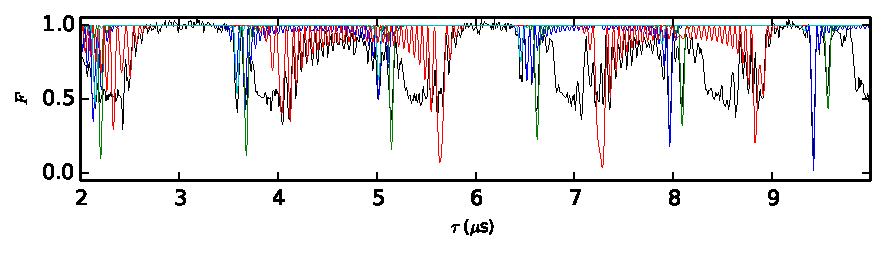
\includegraphics{Img/Truefingerprint.pdf}
    \caption{Fingerprint of Hans Sil01 at B = 304.12G for N=32 pulses.}
    \label{fig:FP}
\end{figure}

\begin{table}[htbp]
    \begin{tabular}{lllll}
    Carbon &  $A_{\parallel} $ & $A_{\perp}$ \\ \hline
    1         & 30.0 kHz$\cdot 2 \pi$             & 80.0 kHz$\cdot 2 \pi$                \\
    2         & 27.0 kHz$\cdot 2 \pi$             & 28.5 kHz$\cdot 2 \pi$              \\
    3         & -51.0 kHz$\cdot 2 \pi$          & 105.0 kHz$\cdot 2 \pi$              \\
    4         & 45.1 kHz$\cdot 2 \pi$           & 20.0 kHz$\cdot 2 \pi$                \\
    \end{tabular}
    \caption{Hyperfine paramters used to fit spins 1 to 4 in \autoref{fig:FP}.}
    \label{tbl:HF_par}
\end{table}

Lorem ipsum dolor sit amet, consectetur adipisicing elit, sed do eiusmod
tempor incididunt ut labore et dolore magna aliqua. Ut enim ad minim veniam,
quis nostrud exercitation ullamco laboris nisi ut aliquip ex ea commodo
consequat. Duis aute irure dolor in reprehenderit in voluptate velit esse
cillum dolore eu fugiat nulla pariatur. Excepteur sint occaecat cupidatat non
proident, sunt in culpa qui officia deserunt mollit anim id est laborum.


\begin{figure}[htbp]
    \centering
    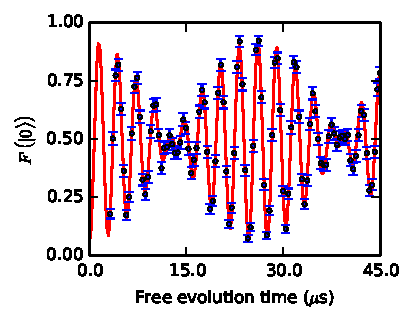
\includegraphics{Img/CarbonRamsey_C1.pdf}
    \caption{Nuclear Ramsey of Carbon 1}
    \label{fig:CR_C1}
\end{figure}

\begin{figure}[htbp]
    \centering
    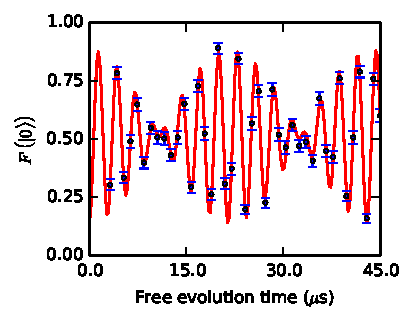
\includegraphics{Img/CarbonRamsey_C4.pdf}
    \caption{Nuclear Ramsey of Carbon 4}
    \label{fig:CR_C4}
\end{figure}

\section{Controlling weakly coupled carbons trough the electronic spin}
% Section containing theory (Gate circuits) on how to initialize and readout carbons





\section{Carbon Initialization \& Readout}
% TODO_MAR: Discuss naming of sec: Carbon Init&RO and Carbon Tomo
%  Section containing experimental results (Tomographies)
%  Should emphasize difficulty in seperating initialization and RO fidelity, what is not working? Is it working?




